%% LyX 2.0.2 created this file.  For more info, see http://www.lyx.org/.
%% Do not edit unless you really know what you are doing.
\documentclass[a4paper,english]{article}
\usepackage[T1]{fontenc}
\usepackage[latin9]{inputenc}
\usepackage{babel}
\usepackage{amsmath}
\usepackage{amssymb}
\usepackage{graphicx}
\usepackage[unicode=true,pdfusetitle,
 bookmarks=true,bookmarksnumbered=false,bookmarksopen=false,
 breaklinks=false,pdfborder={0 0 1},backref=section,colorlinks=false]
 {hyperref}

\makeatletter

%%%%%%%%%%%%%%%%%%%%%%%%%%%%%% LyX specific LaTeX commands.
\pdfpageheight\paperheight
\pdfpagewidth\paperwidth

%% Because html converters don't know tabularnewline
\providecommand{\tabularnewline}{\\}

%%%%%%%%%%%%%%%%%%%%%%%%%%%%%% User specified LaTeX commands.
\usepackage{babel}
\usepackage{a4wide}\usepackage{babel}

\@ifundefined{showcaptionsetup}{}{%
 \PassOptionsToPackage{caption=false}{subfig}}
\usepackage{subfig}
\makeatother

\begin{document}

\section{Methodology}

We model the evolution of color terms as a similarity-maximization
signaling game, in the spirit of JagerXXX. We make, however, a number
of changes to better fit the problem at hand. Quantitative evaluation
is performed against the WCS data by matching simulation results with
actual languages and calculating the quality of the match.


\subsection{Simulation setup}

\label{sub:simulation}

First of all, we use Munsell chips as individual percepts and define
their distance in terms of their coordinates in CIELAB color space,
as is done by RegierXXX. This constitutes the perceptual space to
be used in the game. In order to somewhat simplify modeling and implementation,
we decided to ignore the 10 achromatic chips used in the WCS. Therefore,
the perceptual space consists of 320 points. These can be indexed
by hue (40 levels) and value (8 levels) or by coordinates in CIELAB
space $L$, $a$, $b$. We used the mapping from hue and value to
CIELAB space provided with the WCS data%
\footnote{Obtained from \href{http://www1.icsi.berkeley.edu/wcs/data/cnum-maps/cnum-vhcm-lab-new.txt}{http://www1.icsi.berkeley.edu/wcs/data/cnum-maps/cnum-vhcm-lab-new.txt}(accessed
17/01/2013).%
}. Given two points $x_{1}=\left\langle L_{1},a_{1},b_{1}\right\rangle $
and $x_{2}=\left\langle L_{2},a_{2},b_{2}\right\rangle $, their similarity
is given by: 
\[
sim\left(x_{1},x_{2}\right)=e^{-c\times\left(dist\left(x_{1},x_{2}\right)\right)^{2}}
\]
 where $dist\left(x_{1},x_{2}\right)$ is the euclidean distance in
CIELAB space: 
\[
dist\left(x_{1},x_{2}\right)=\sqrt{\left(L_{1}-L_{2}\right)^{2}+\left(a_{1}-a_{2}\right)^{2}+\left(b_{1}-b_{2}\right)^{2}}
\]
 To be in line with RegierXXX we use $c=0.001$ for all simulations.

The similarity-maximization game consists of the tuple $\left\langle T,\Pr,M,U\right\rangle $,
where $T$ is the perceptual space described above, $\Pr\in\Delta\left(T\right)$
is a probability distribution over $T$, $M$ is the set of messages
available, and $U\in T\times T\rightarrow\mathbb{R}$ is the utility
function for both speaker and hearer. We define only one utility function
for both speaker and hearer, thus we assume perfectly cooperative
interests. Furthermore, we assume that talk is cheap and utility is
directly proportional to similarity, \emph{i.e.}\ $U\left(x_{1},x_{2}\right)=sim\left(x_{1},x_{2}\right)$.

Regarding solution concepts for the game, we use replicator dynamics
over mixed strategies. A sender strategy $\sigma\in T\rightarrow\Delta\left(M\right)$
associates to each point in the perceptual space a probability distribution
over the set of messages. A receiver strategy $\rho\in M\rightarrow\Delta\left(T\right)$
associates to each message a probability distribution over all points
in perceptual space. Probability values should be interpreted as percentages
of a hypothetical population. Therefore, if $\sigma\left(x_{1},m_{1}\right)=0.7$
this should be interpreted as ``$70\%$ of the population uses message
$m_{1}$ when observing point $x_{1}$''. The dynamics update these
strategies according to their expected utility. The state of each
strategy at time instant $t+1$ is defined as follows: 
\[
\sigma_{t+1}\left(x,m\right)=\sigma_{t}\left(x,m\right)\times\frac{\textnormal{EU}_{\sigma_{t}}\left(m\mid x,\rho_{t}\right)\times\left|M\right|}{\underset{m^{\prime}\in M}{\sum}\textnormal{EU}_{\sigma_{t}}\left(m^{\prime}\mid x,\rho_{t}\right)}
\]
 
\[
\rho_{t+1}\left(m,x\right)=\rho_{t}\left(m,x\right)\times\frac{\textnormal{EU}_{\rho_{t}}\left(x\mid m,\sigma_{t}\right)\times\left|T\right|}{\underset{x^{\prime}\in T}{\sum}\textnormal{EU}_{\rho_{t}}\left(x^{\prime}\mid m,\sigma_{t}\right)}
\]
 where expected utilities are defined as: 
\[
\textnormal{EU}_{\sigma}\left(m\mid x,\rho\right)=\underset{x^{\prime}\in T}{\sum}\rho\left(x^{\prime}\mid m\right)\times U\left(x,x^{\prime}\right)
\]
 
\[
\textnormal{EU}_{\rho}\left(x\mid m,\sigma\right)=\underset{x^{\prime}\in T}{\sum}\Pr\left(x^{\prime}\right)\times\sigma\left(m\mid x^{\prime}\right)\times U\left(x^{\prime},x\right)
\]
 Starting conditions $\sigma_{0}$ and $\rho_{0}$ are initialized
with random values for every simulation. All simulations were ran
until a convergence criterion was met. The criterion was that the
total absolute change in both sender and receiver strategy was under
$1\%$, \emph{i.e.}: 
\begin{eqnarray*}
 & \underset{x\in T}{\sum}\underset{m\in M}{\sum}\left|\sigma_{t+1}\left(x,m\right)-\sigma_{t}\left(x,m\right)\right|<0.01\\
 & \wedge\\
 & \underset{m\in M}{\sum}\underset{x\in T}{\sum}\left|\rho_{t+1}\left(m,x\right)-\rho_{t}\left(m,x\right)\right|<0.01
\end{eqnarray*}



\subsection{Quantitative evaluation}

\label{sub:quantitative-evaluation}

Following the approach by RegierXXX, we calculated a mode map per
language in the WCS data. Each language was then classified regarding
the number of main color terms. Since RegierXXX did not provide a
clear criterion for what they consider a main color term, we employed
our own heuristic: we counted for each language how many color terms
cover at least $5\%$ of the space, \emph{i.e.}\ at least $16$ Munsell
chips.

We can then try to match two $n$-term languages (or simulation results)
$L_{1}$ and $L_{2}$ by mapping terms in one language to terms in
the other. The procedure was to establish the mapping based on the
amount of overlap between terms as follows: 
\begin{enumerate}
\item Calculate, for each pair of terms $t_{1}\in L_{1}$ and $t_{2}\in L_{2}$,
the number of chips they both cover; 
\item Establish a one-to-one mapping starting with the two terms that have
the highest overlap until no more terms are left or no overlap exists
between the remaining terms. 
\end{enumerate}
The quality of each pairing can be calculated in terms of precision
and recall, \emph{i.e.}\ what percentage of $t_{1}$ chips are also
$t_{2}$ and what percentage of $t_{2}$ chips are also $t_{1}$.
The overall quality of the mapping can be calculated in terms of accuracy,
\emph{i.e.}\ what percentage of total overlap is there with the established
mapping.

The accuracy numbers can then be summarized to give an impression
of the overall match between languages (or simulation results) and
the languages in the WCS. As reference points for comparison we calculated
these numbers not only for our simulation results but for three other
scenarios, namely: 
\begin{enumerate}
\item Matching each WCS language against its peers (in number of main color
terms). This establishes a pragmatic upper bound to how well we can
expect a simulation to be able to perform; 
\item Simulation results performed with a neutral similarity metric. Since
the Munsell chips are distributed in CIELAB space as a irregular sphere,
for these results we laid them out as a regular sphere. For that we
used as spherical coordinates, value to indicate the elevation angle,
hue to indicate the azimuth angle, and a fixed radius estimated from
the irregular sphere. Distance was then computed by converting these
coordinates to Cartesian coordinates and calculating the Euclidean
distance; 
\item Random assignment of color terms to chips (basically the initial conditions
of the simulation). This establishes a lower bound for comparison. 
\end{enumerate}

\section{Results}


\subsection{Quantitative evaluation}

As described in Section~\ref{sub:quantitative-evaluation} all languages
in the WCS were classified in terms of their number of main color
terms. The following table summarizes the results. These do not correspond
to those reported by KayXXX since the criteria used are not the same.

\begin{center}
\begin{tabular}{r|rrrrrr}
Number of main color terms  & 3  & 4  & 5  & 6  & 7  & 8\tabularnewline
\hline 
Number of languages  & 6  & 12  & 31  & 40  & 14  & 7 \tabularnewline
\end{tabular}
\par\end{center}

Based on these results, we ran $10$ simulations for each of the number
of color terms, and established mappings between each of the outcomes
and the languages in the WCS in the respective categories. For example,
for $3$ terms we have $10$ simulations matched against $6$ languages,
thus $60$ accuracy values. Table~\ref{tab:overall-statistics} contains
the overall statistics for each number of terms and for each scenario.
We illustrate these numbers in Figure~\ref{fig:plots} with the simulations
involved in the best and worst matches.

\begin{table}
\begin{centering}
\begin{tabular}{rrrrrrrl}
\hline 
$n$  & Min.  & 1st Qu.  & Median  & Mean  & 3rd Qu.  & Max.  & \tabularnewline
\hline 
3  & 0.779  & 0.833  & 0.870  & 0.865  & 0.909  & 0.930  & \tabularnewline
4  & 0.336  & 0.545  & 0.630  & 0.629  & 0.712  & 0.836  & \tabularnewline
5  & 0.373  & 0.603  & 0.700  & 0.688  & 0.776  & 0.900  & \tabularnewline
6  & 0.400  & 0.606  & 0.679  & 0.670  & 0.739  & 0.879  & \tabularnewline
7  & 0.379  & 0.521  & 0.588  & 0.600  & 0.673  & 0.818  & \tabularnewline
8  & 0.488  & 0.600  & 0.715  & 0.690  & 0.741  & 0.888  & \tabularnewline
\hline 
3  & 0.394  & 0.468  & 0.602  & 0.583  & 0.692  & 0.788  & \tabularnewline
4  & 0.324  & 0.479  & 0.552  & 0.547  & 0.606  & 0.761  & \tabularnewline
5  & 0.388  & 0.500  & 0.533  & 0.542  & 0.573  & 0.703  & \tabularnewline
6  & 0.364  & 0.455  & 0.497  & 0.501  & 0.545  & 0.661  & \tabularnewline
7  & 0.376  & 0.458  & 0.486  & 0.489  & 0.521  & 0.630  & \tabularnewline
8  & 0.361  & 0.447  & 0.476  & 0.492  & 0.548  & 0.664  & \tabularnewline
\hline 
3  & 0.421  & 0.533  & 0.579  & 0.573  & 0.618  & 0.703  & \tabularnewline
4  & 0.324  & 0.412  & 0.458  & 0.457  & 0.495  & 0.591  & \tabularnewline
5  & 0.261  & 0.400  & 0.452  & 0.447  & 0.486  & 0.600  & \tabularnewline
6  & 0.285  & 0.412  & 0.442  & 0.441  & 0.476  & 0.573  & \tabularnewline
7  & 0.318  & 0.418  & 0.448  & 0.444  & 0.473  & 0.570  & \tabularnewline
8  & 0.327  & 0.405  & 0.427  & 0.425  & 0.447  & 0.509  & \tabularnewline
\hline 
3  & 0.321  & 0.342  & 0.348  & 0.350  & 0.355  & 0.379  & \tabularnewline
4  & 0.224  & 0.270  & 0.285  & 0.282  & 0.294  & 0.321  & \tabularnewline
5  & 0.182  & 0.224  & 0.233  & 0.234  & 0.245  & 0.270  & \tabularnewline
6  & 0.164  & 0.203  & 0.212  & 0.214  & 0.224  & 0.258  & \tabularnewline
7  & 0.155  & 0.179  & 0.191  & 0.190  & 0.200  & 0.239  & \tabularnewline
8  & 0.148  & 0.170  & 0.179  & 0.179  & 0.188  & 0.221  & \tabularnewline
\hline 
\end{tabular}
\par\end{centering}

\caption{Summary statistics of match accuracy against languages in the WCS.}


\label{tab:overall-statistics} 
\end{table}


\begin{figure}
\subfloat[Simulation with one of the best average accuracy values: 0.715. Best
match against \ref{fig:kwerba}. Worst match against \ref{fig:nafaanra}.]{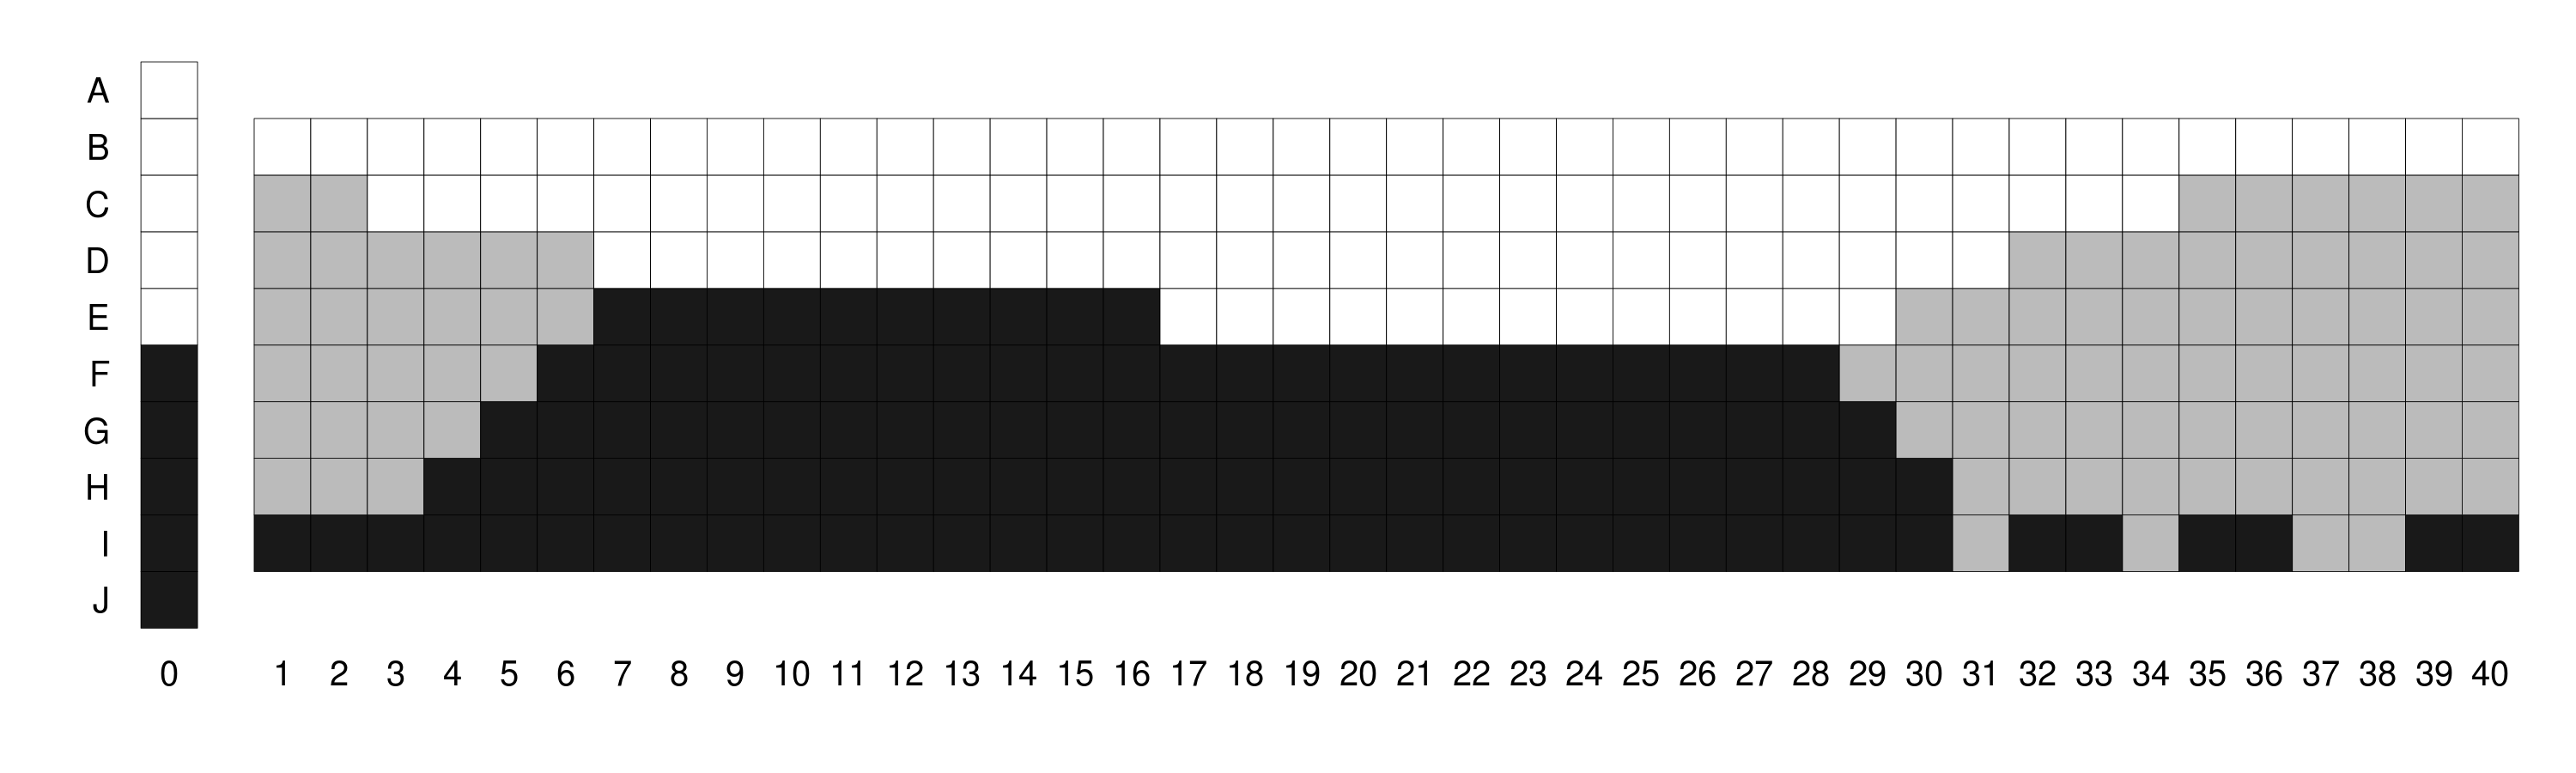
\includegraphics[width=0.48\textwidth]{3-2}

\label{fig:best-simulation}

}\hfill{}\subfloat[Simulation with one of the worst average accuracy values: 0.449. Best
match against \ref{fig:chacobo}. Worst match against \ref{fig:culina}.]{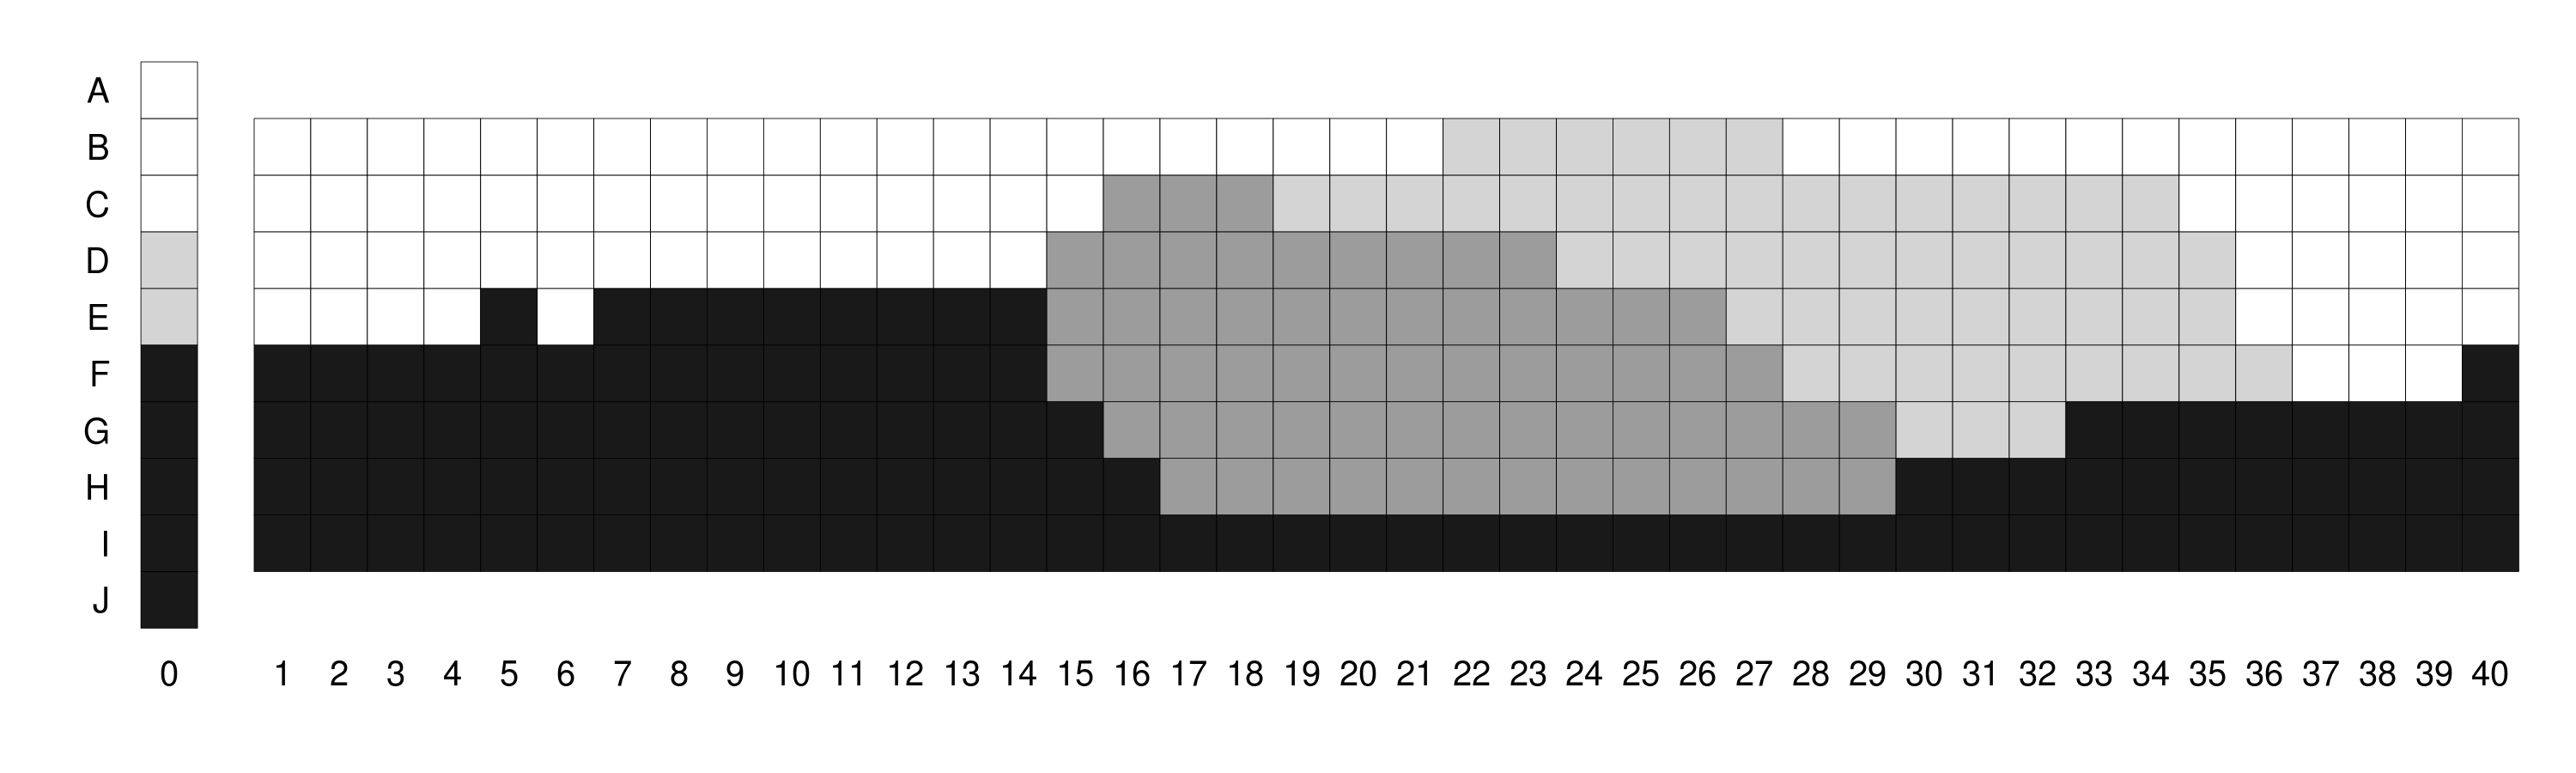
\includegraphics[width=0.48\columnwidth]{4-2}

\label{fig:worst-simulation}

}

\subfloat[Kwerba language. Average within-category accuracy: 0.815. Match accuracy
against \ref{fig:best-simulation}: 0.788.]{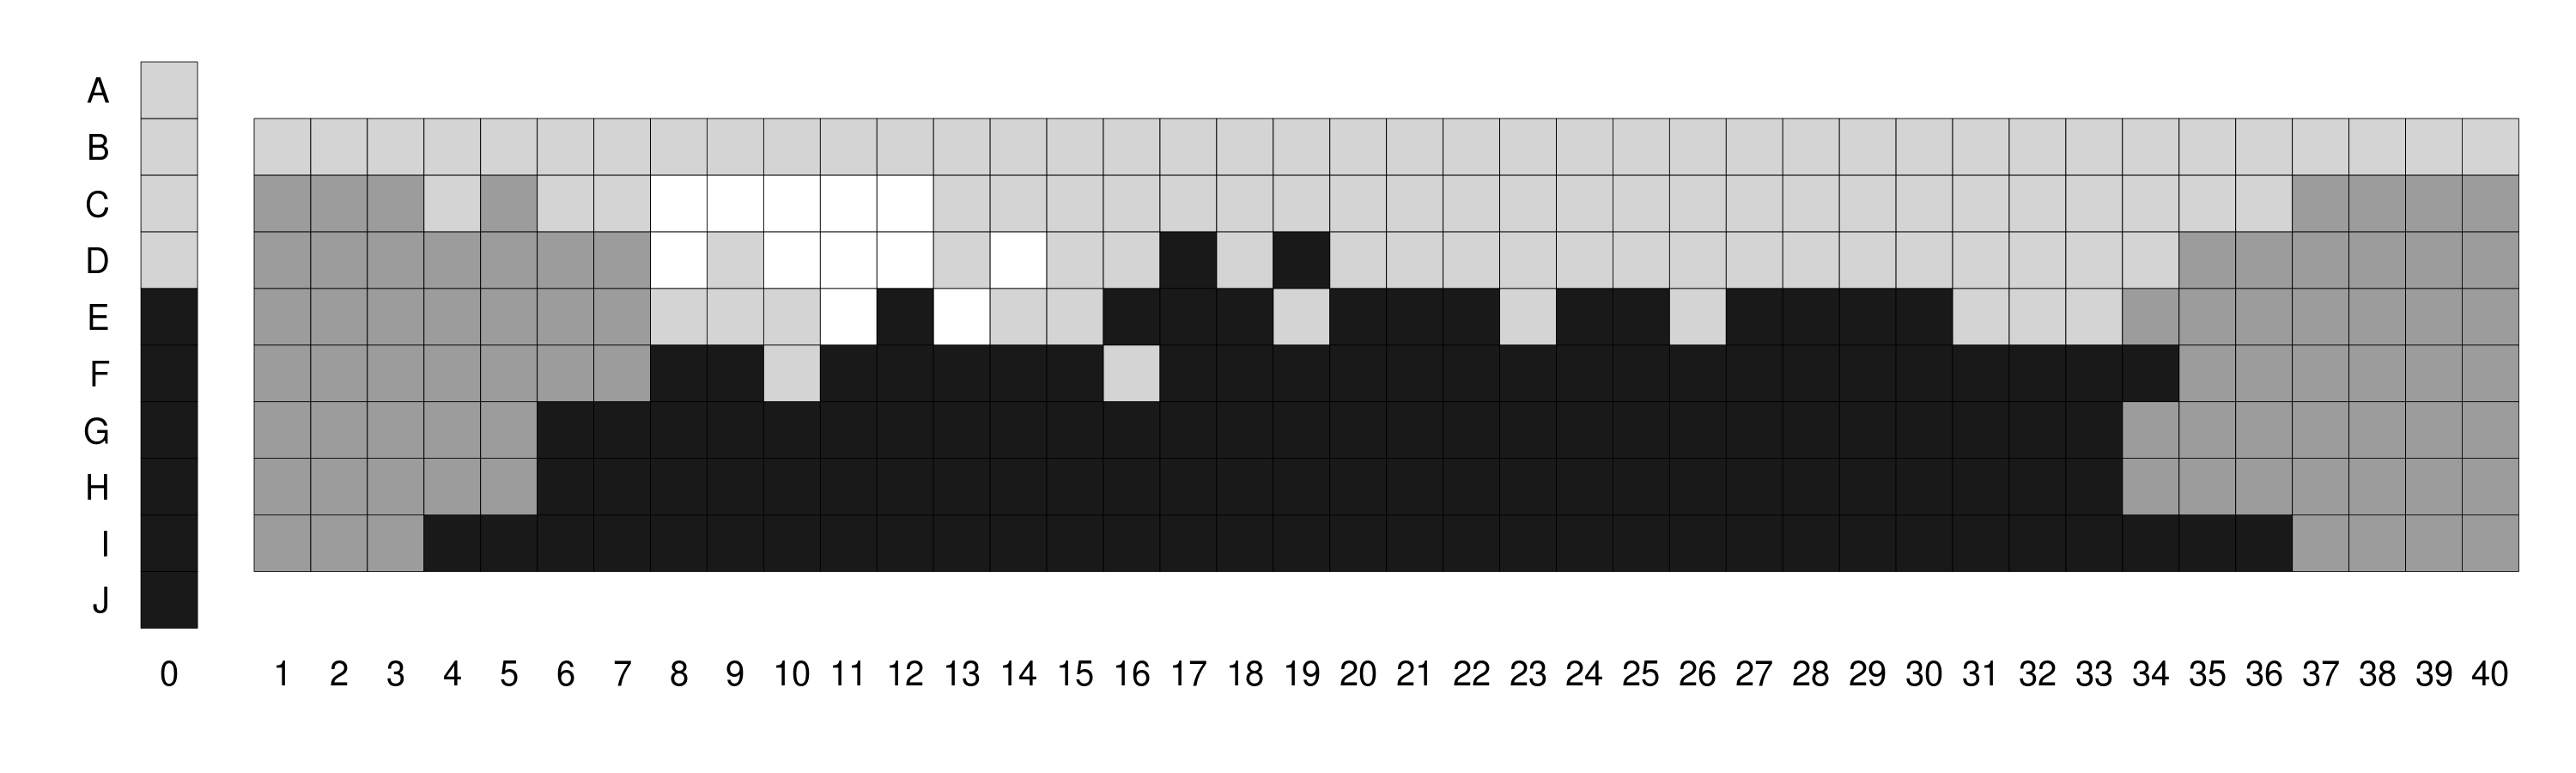
\includegraphics[width=0.48\columnwidth]{Kwerba}

\label{fig:kwerba}

}\hfill{}\subfloat[Ch�cobo language. Average within-category accuracy: 0.690. Match with
\ref{fig:worst-simulation}: 0.524.]{\includegraphics[width=0.48\columnwidth]{Ch�cobo}

\label{fig:chacobo}

}

\subfloat[Nafaanra language. Average within-category accuracy: 0.870. Match
with \ref{fig:best-simulation}: 0.658. Match with \ref{fig:kwerba}:
0.779.]{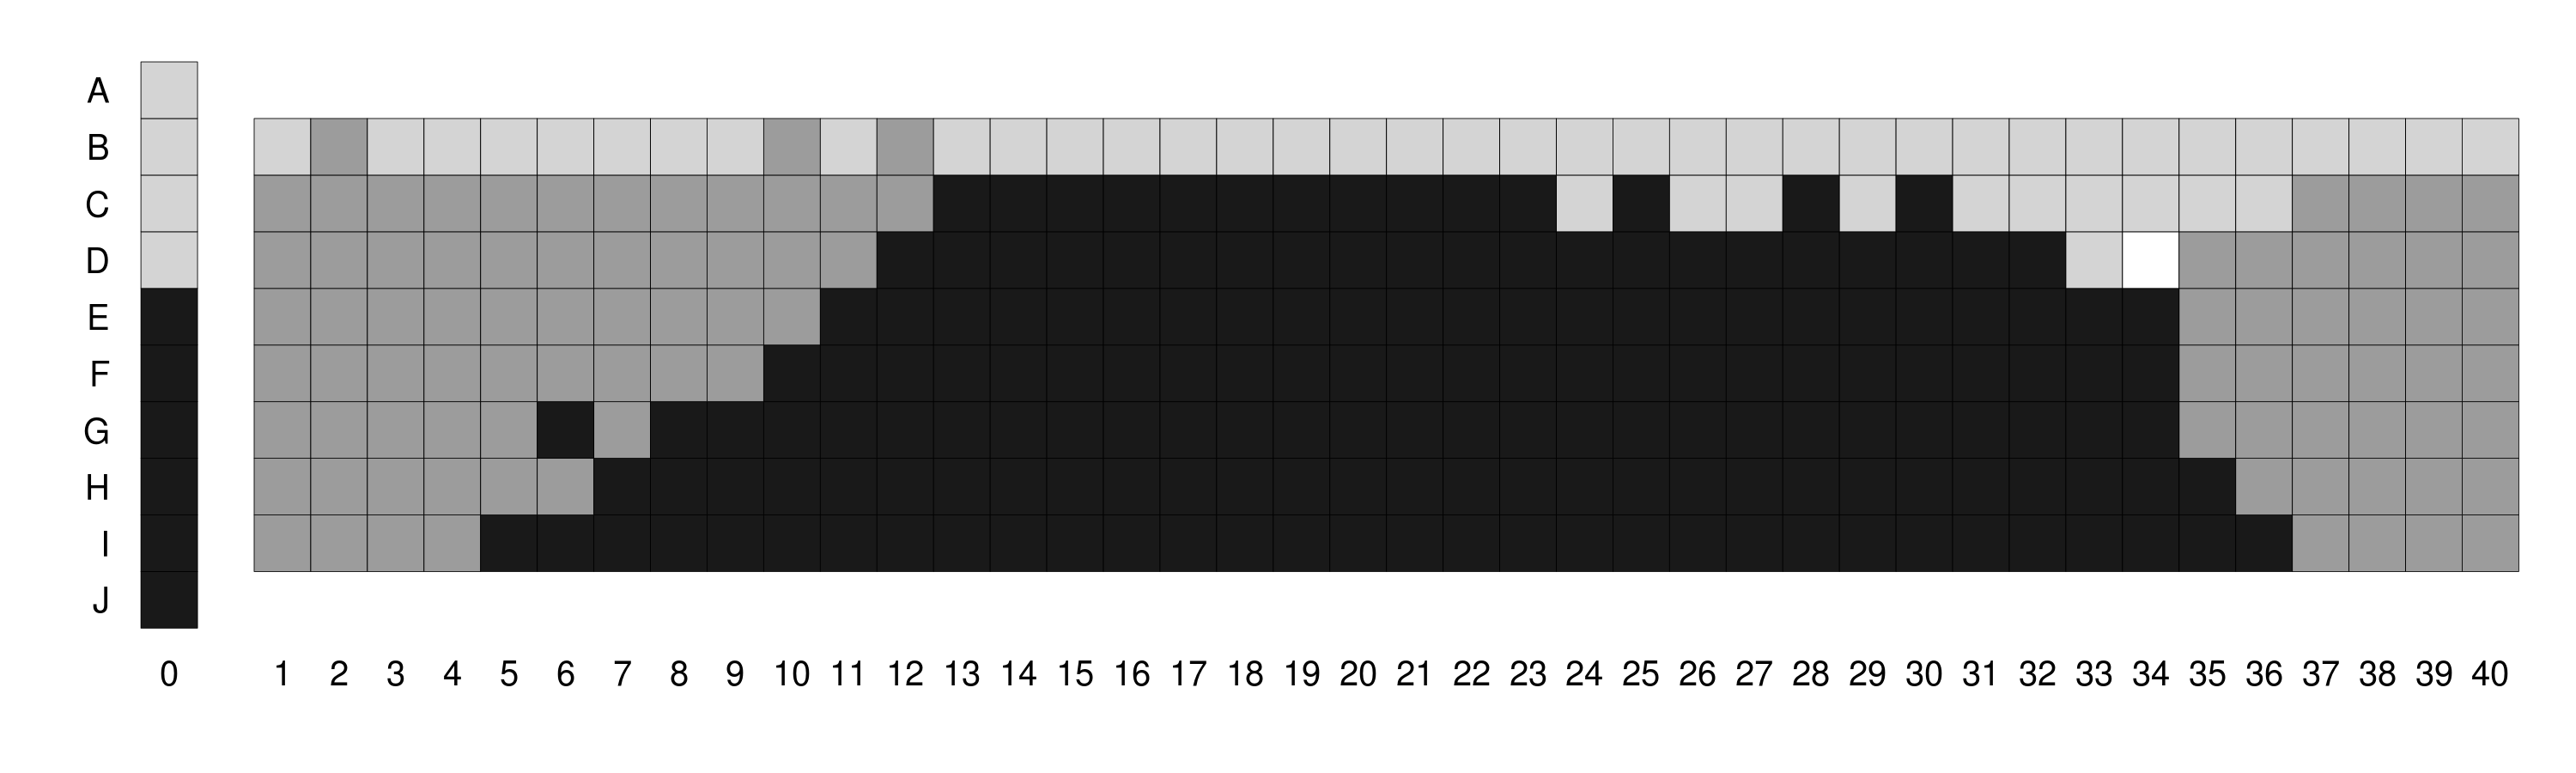
\includegraphics[width=0.48\columnwidth]{Nafaanra}

\label{fig:nafaanra}

}\hfill{}\subfloat[Culina language. Average within-category accuracy: 0.595. Match with
\ref{fig:worst-simulation}: 0.324. Match with \ref{fig:chacobo}:
0.564.]{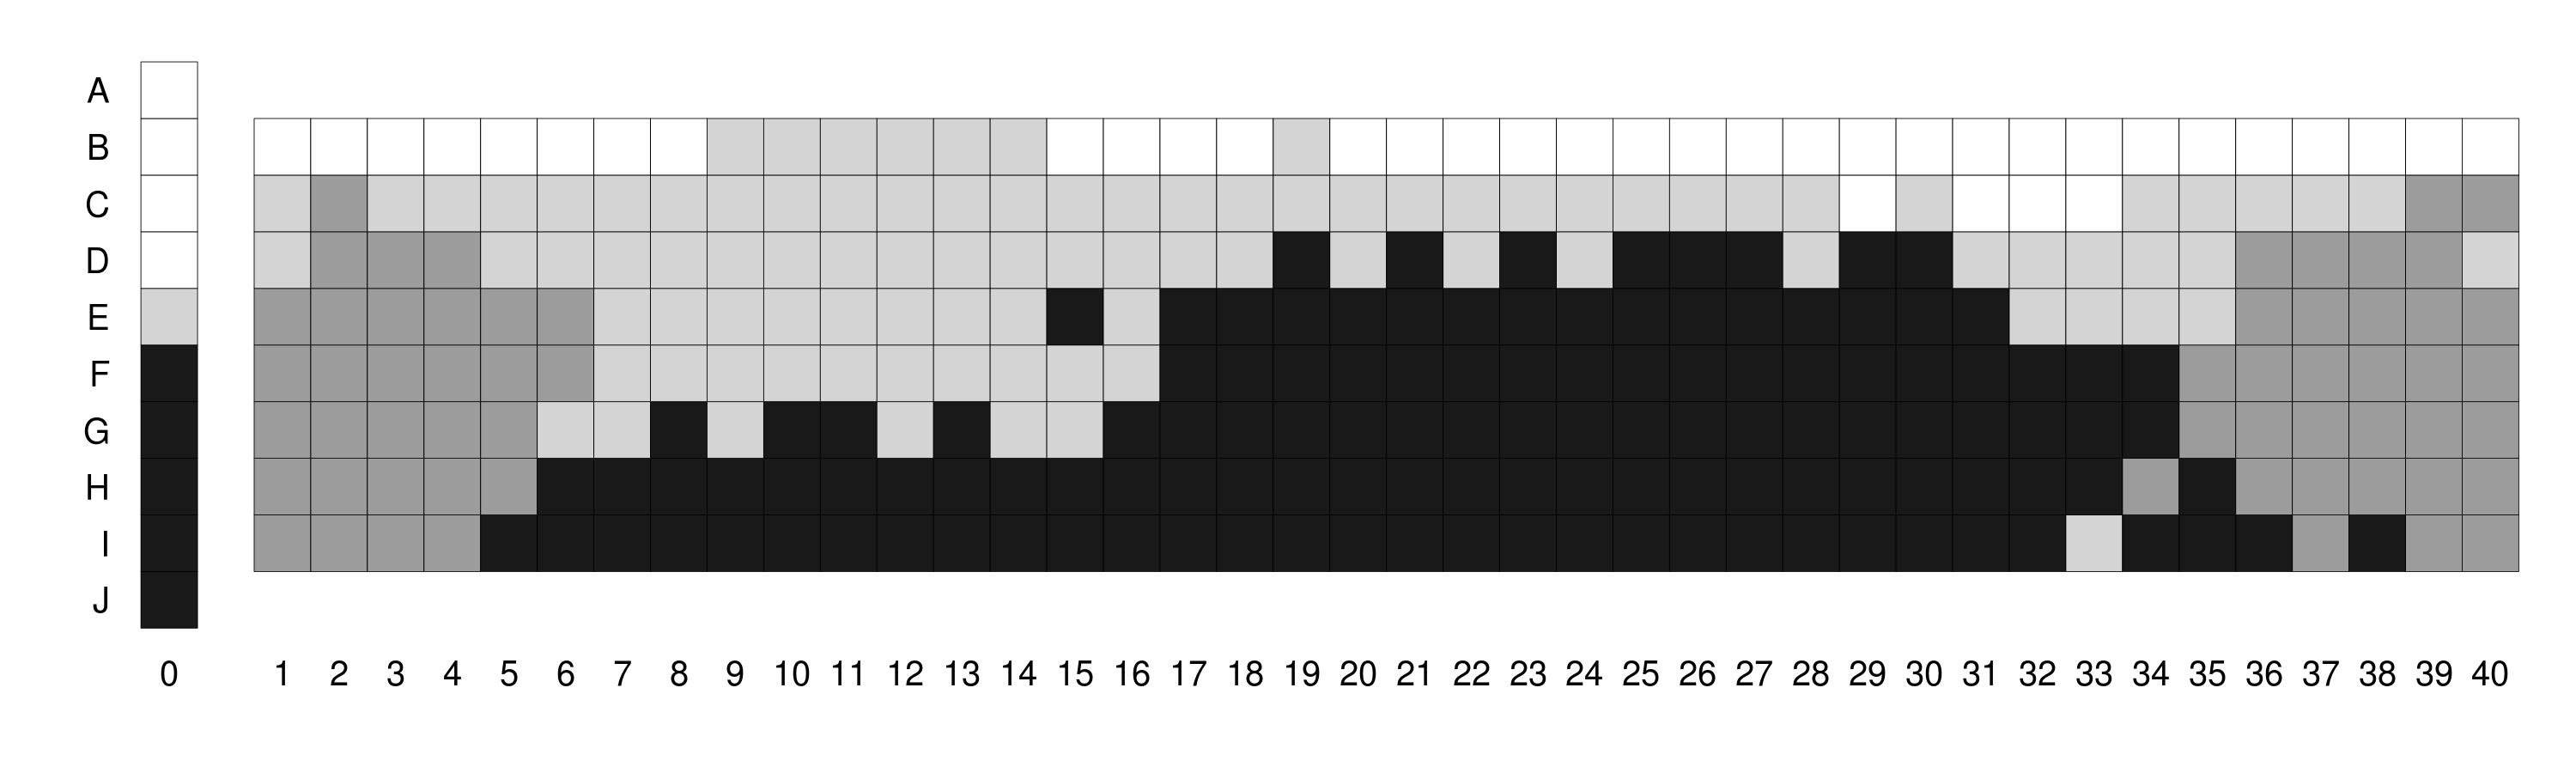
\includegraphics[width=0.48\columnwidth]{Culina}

\label{fig:culina}

}

\caption{Simulation results and matches with WCS languages.}
\label{fig:plots}
\end{figure}


What the numbers indicate is that the simulations are approximating
the phenomenon, although in a limited way. As expected, the accuracy
values obtained by the simulation results are significantly higher
than those obtained by random assignment. However, they are also significantly
lower than the within-category accuracy values obtained by the languages
in the WCS, albeit closer to this scenario than to the random one.
The comparison with the perfect sphere scenario shows how important
the topology of the color space is: the accuracy values for this scenario
are quite close to the ones obtained by the simulation results. However,
they are also consistently lower, which indicates that our simulation
setup is capturing some other non-trivial characteristics of the phenomenon.
\end{document}
